\documentclass[12pt]{article}

% Packages
\usepackage[utf8]{inputenc}
\usepackage[czech]{babel}
\usepackage{a4wide}
\usepackage{graphicx}
\usepackage{fancyhdr}
\usepackage{indentfirst}

% Settings
\newcommand{\Title}{Obsah a forma konsolidované účetní závěrky}
\newcommand{\Author}{Čermák Jan, Drahuský Marek, Ďurčová Simona,\\
Knapová Kristýna, Knobová tereza}
% Page style
\pagestyle{fancy}
\linespread{1.5}

% Title page
\title{\Title}
\author{\Author}
\date{}

% Header and footer
\fancyhf{}
\renewcommand{\headrulewidth}{0.4pt}
\renewcommand{\footrulewidth}{0.4pt}
\lhead{\Title}
\rhead{\Author}
\lfoot{\today}
\rfoot{\thepage}

\begin{document}

% First page without number of page
\maketitle
\thispagestyle{empty}

\section{Úvod}
Konsolidovaná účetní závěrka představuje účetní závěrku sestavenou za skupinu kapitálově 
provázaných podniků, které tvoří jeden ekonomický celek. Její funkcí je informovat investory 
podniků ve skupině, případně další uživatele účetních informací o majetkové a finanční pozici 
celé skupiny, jako by šlo o jediný podnik. Při jejím sestavení jsou tedy agregovány údaje 
o majetku, finanční situaci a hospodářském výsledku jednotlivých právních subjektů 
zahrnutých do konsolidačního celku, při eliminaci všech vztahů uvnitř celku.  Konsolidovaná účetní závěrka musí být ověřena auditorem.
\\

Zákon o účetnictví stanovuje povinnost sestavit konsolidovanou účetní závěrku konsolidující účetní jednotce – tedy takové jednotce, která je obchodní společností a je řídící osobou nebo ovládající osobou.
\\
Konsolidovanou účetní závěrku tvoří: 
\begin{itemize}
\item rozvaha (bilance), 
\item výkaz zisku a ztráty, 
\item příloha včetně přehledu o peněžních tocích. 
\end{itemize}
Konsolidaci lze uskutečňovat podle příslušné konsolidační metody, a to buď způsobem přímé konsolidace, nebo konsolidace postupné po jednotlivých úrovních dílčích konsolidačních celků. 
\\

Přímou konsolidací se rozumí konsolidace všech účetních jednotek konsolidačního 
celku najednou.
\\

Konsolidace po jednotlivých úrovních dílčích konsolidačních celků. Dochází k postupné konsolidaci po jednotlivých úrovních. Tento postup konsolidace je označován jako konsolidace postupná. 
\\

Jednou zvolený způsob konsolidace se nemá měnit a má být důsledně a trvale používán u účetních jednotek, které tvoří konsolidační celek. 


\section{Metody konsolidace} 
\begin{itemize}
\item metoda plné konsolidace
\item metoda ekvivalence
\item metoda poměrné konsolidace
\end{itemize}

\subsection{Metoda plné konsolidace}

Metoda plné konsolidace vychází z předpokladu dominantního postavení mateřského podniku nad dceřiným podnikem, prostřednictvím něhož mateř. podnik rozhoduje o veškerém majetku a závazcích bez ohledu na to, že nedrží 100% podíl na ZK u dceřiného podniku.
 
\subsection{Metoda ekvivalence}

Metoda ekvivalence předpokládá, že mateřský podnik uplatňuje v přidruženém pouze podstatný vliv, tj. nekontroluje ho v plné míře. Je postavena na principu přecenění cenných papírů, jejichž emitentem je přidružený podnik poměrnou částí vlastního jmění tohoto podniku.
\\

V České republice je tato metoda zařazena mezi konsolidační metody. Některé země 
i mezinárodní účetní standardy však ekvivalenční metodu za konsolidační metodu nepovažují.

\subsection{Metoda poměrné konsolidace}

Poměrná konsolidace - použije se při zahrnutí podniku, který je celý ovládán ve shodě s dalšími podniky, pokud tyto podniky mají shodný podíl na základním kapitálu ovládaného podniku,

\section{Etapy}

Celý proces konsolidace probíhá ve čtyřech fázích (etapách):
\subsection{První fáze}
V první fází je nutné vymezit potenciální konsolidační celek, který se skládá z mateřského podniku, dceřiných a přidružených podniků. Mateřský podnik - podnik, který drží v jiném podniku 20 a více \% podíl na ZK Dceřiný podnik - podnik, ve kterém mateř. podnik uplatňuje přímo nebo nepřímo rozhodující vliv, tj. vlastní více než 50 \% akcií či podílů na ZK Přidružený podnik - podnik, ve kterém mateřský uplatňuje podstatný vliv, tj. drží min. 20 \% a max. 50 \% podílu na ZK.
\\

Osvobozeny od povinnosti sestavovat konsolidovanou účetní závěrku jsou podniky, které účtují podle jiné osnovy a postupů účtování, vstupují do likvidace, konkurzu nebo vyrovnání, mají sídlo na území jiného státu a nedosáhly alespoň dvou ze tří stanovených kritérií (podle zákona o účetnictví):

\begin{itemize}

\item výše čistého obratu činila více než 700 mil. Kč
\item výše jejich brutto aktiv činila více než 350 mil. Kč
\item průměrný přepočtený stav zaměstnanců více než 250.

\end{itemize}
Konsolidovaná účetní závěrka se sestavuje na podkladě účetních závěrek podniku mateřského, dceřiného a přidruženého za příslušné účetní období ke dni účetní závěrky mateřského podniku. Potenciální konsolidační celek se po provedení všech úprav testuje, zda jsou splněny výše uvedené podmínky.
\\

\subsection{Druhá fáze}
V druhé fází probíhá:
\begin{itemize}
\item analýza vztahů mezi podniky konsolidačního celku
\item určení konsolidačních metod a systému konsolidace
\item stanovení konsolidačních pravidel (sestavuje je a vyhlašuje mateř. podnik - úprava položek rozvahy a výsledovky, popis oceňování majetku a závazků, volba přepočtu kurzových rozdílů, způsob odepisování apod.)
\end{itemize}

\subsection{Třetí fáze}
Třetí fáze je prováděcí, tj. nastává:

\begin{itemize}
\item přetřídění účtů mateřského podniku
\item vypořádání rozdílu po první konsolidaci
\item vyloučení cenných papírů a vkladů a jejich nahrazení podílem na vlastním jmění přidruženého podniku
\item vypořádání HV přidruženého podniku za běžné účetní období
\item akumulované HV minulých let
\end{itemize}


\subsection{Čtvrtá fáze}
Čtvrtá fáze je závěrečná, tj. nastává:

\begin{itemize}
\item sestavení konsolidované rozvahy, výsledovky a přílohy
\item zveřejnění údajů
\item audit
\end{itemize}


Význam a důsledek konsolidace:
\\
\begin{figure}[h]
\begin{center}
	\caption{Význam a důsledek konsolidace}
		\label{figure:vyznam-dusledek}
		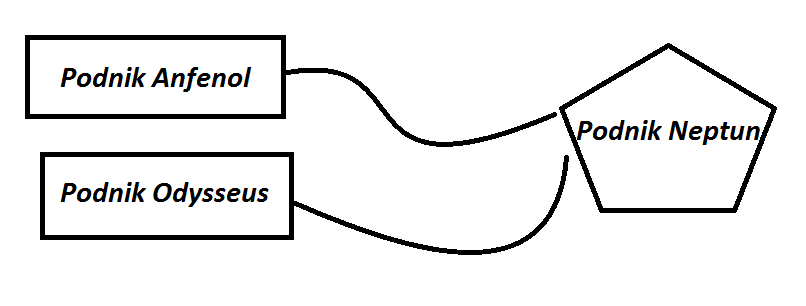
\includegraphics[scale=0.8]{pics/1-vyznam-dusledek.png}
	\end{center}
\end{figure}
\\
\subsection{Akvizice z hlediska účetního}

\begin{figure}[h]
\begin{center}
	\caption{Akvizice z hlediska účetního}
		\label{figure:ucetni-vyznam}
		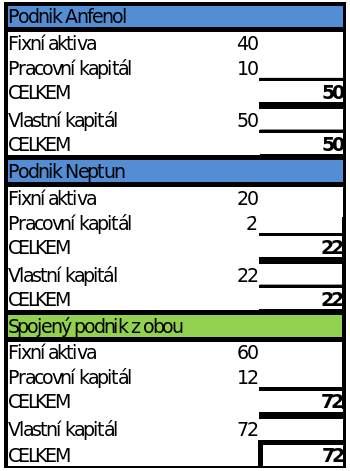
\includegraphics[scale=0.6]{pics/2-tabulka.png}
	\end{center}
\end{figure}

Akvizici lze z účetního pohledu provést koupí nebo vkladem podílů. V praktickém příkladu prvý podnik získá druhý, nový podniku vlastní společně všichni akcionáři obou dříve nezávislých podniků. Celkový majetek se nezmění a účetně nevzniká pozitivní rozdíl mezi kupní cenou podniku a reálnou cenou kupovaného podniku.\\

Případová studie k vysvětlení základního účetního principu konsolidace:\\
Dispozice:\\
Podnik Anfenol koupil 100  \% podniku Odysseus, a to k rozvahovému dni obou podniků 3.prosince 2012.
\\
\\
Přehled bilančních polože ukazuje obrázek 3.
\begin{figure}[!h]
\begin{center}
	\caption{Přehled bilančních položek}
		\label{figure:prehled-bilancnich-polozek}
		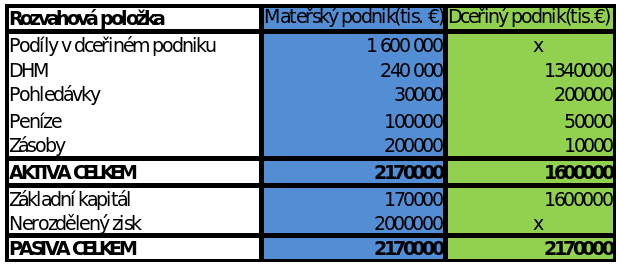
\includegraphics[scale=0.58]{pics/3-tabulka.png}
	\end{center}
\end{figure}
\\

\section{Proces konsolidace}

\begin{figure}[h]
\begin{center}
	\caption{Proces konsolidace}
		\label{figure:proces-konsolidace}
		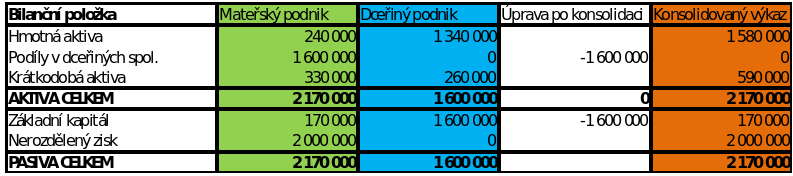
\includegraphics[scale=0.6]{pics/4-tabulka.png}
	\end{center}
\end{figure}

Sestavení konsolidované rozvahy probíhá podle následujících pravidel:
\begin{enumerate}
\item Jednotlivé účetní rozvahy je nutno připravit tak, aby byla sestavena dle stejných účetních pravidel.
\item Vyloučit pořizovací cenu investic proti vlastníkům kapitálu dceřiného podniku a uznat goodwill z pořízení podílu v dceřiném podniku.
\item Sečíst veškerá aktiva i pasiva mateřského i dceřiných podniků v plné výši.
\item Provést úpravy o vnitropodnikové transakce.
\item Základní kapitál je vždy základním kapitálem mateřského podniku.
\item Nakonec vykázat menšinové podíly. 
\end{enumerate}
\end{document}